\documentclass{standalone}
\usepackage{pgfplots}
\pgfplotsset{soldot/.style={color=black,only marks,mark=*},
             holdot/.style={color=black,fill=white,only marks,mark=*},
             compat=1.12}
\begin{document}
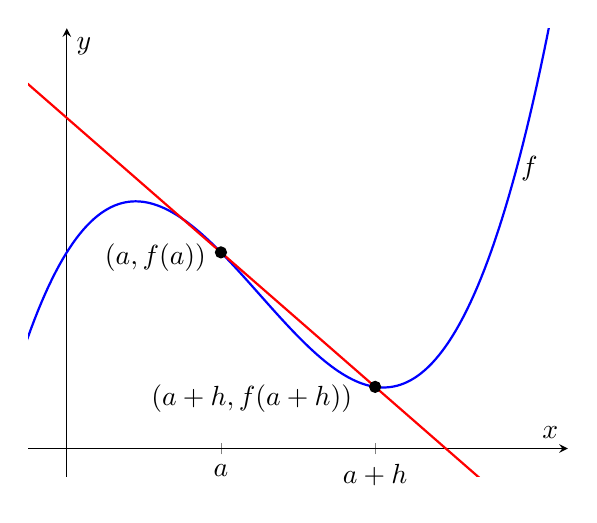
\begin{tikzpicture}
\begin{axis}[
 axis lines=middle,
 %ticklabel style={fill=blue!5!white},
 xmin=-.5,xmax=6.5,
 ymin=-.5,ymax=7.5,
 xtick={2,4},xticklabels={\(a\),\(a+h\)},
 ytick={0},          %<--
% minor tick = {-5,-3,...,5}, %<--
 xlabel=\(x\),ylabel=\(y\),
 samples=200]

\addplot[domain=-2:7,thick,blue] {.2*(x+.5)*(x-3)*(x-5)+2};
\addplot[domain=-2:7,thick,red] {-1.2*(x-2)+3.5};
\addplot[soldot] coordinates{(2,3.5)(4,1.1)};

\draw [] (axis cs:6,5)  node [] {$f$};
\draw [] (axis cs:1.15,3.4)  node [] {$(a,f(a))$};
\draw [] (axis cs:2.4,.9)  node [] {$(a+h,f(a+h))$};

\end{axis}
\end{tikzpicture}
\end{document}